\documentclass[10pt,a4paper,onecolumn]{article}
% \usepackage[utf8]{inputenc}
\usepackage{marginnote}
\usepackage{graphicx}
\usepackage{xcolor}
\usepackage{authblk,etoolbox}
\usepackage{titlesec}
\usepackage{calc}
\usepackage{hyperref}
\hypersetup{breaklinks=true,
            bookmarks=true,
            pdfauthor=
{
		Romain Cazé,
		Marcel Stimberg,
		Benoît Girard
  },
            pdftitle=
{
[Re] Non-additive coupling enables propagation of synchronous spiking activity in purely random networks
},
            colorlinks=true,
            citecolor=blue,
            urlcolor=blue,
            linkcolor=blue,
            pdfborder={0 0 0}}
\urlstyle{same}
\usepackage{tcolorbox}
\usepackage{ragged2e}
\usepackage{fontspec}
\usepackage{fontawesome}
\usepackage{caption}
\usepackage{listings}
\usepackage{siunitx}
\newcommand{\blau}[1]{{\color{blue} #1}}
\newcommand{\rot}[1]{{\color{red} #1}}

\lstnewenvironment{code}{\lstset{language=Python,basicstyle=\small\ttfamily,showstringspaces=false,stringstyle=\color{blue},commentstyle=\color{blue},columns=spaceflexible}}{}



%\usepackage{fancyvrb}
%\VerbatimFootnotes
%\usepackage{graphicx}
%\usepackage{mdframed}
%\newmdenv[backgroundcolor=lightgray]{Shaded}


\usepackage{longtable,booktabs}

\usepackage[
  backend=biber,
%  style=alphabetic,
%  citestyle=numeric
]{biblatex}
\bibliography{biblio.bib}

% --- Macros ------------------------------------------------------------------
\renewcommand*{\bibfont}{\small \sffamily}

\definecolor{red}{HTML}{CF232B}
\newcommand{\ReScience}{Re{\bfseries \textcolor{red}{Science}}}

\newtcolorbox{rebox}
   {colback=blue!5!white, colframe=blue!40!white,
     boxrule=0.5pt, arc=2pt, fonttitle=\sffamily\scshape\bfseries,
     left=6pt, right=20pt, top=6pt, bottom=6pt}

\newtcolorbox{repobox}
   {colback=red, colframe=red!75!black,
     boxrule=0.5pt, arc=2pt, left=6pt, right=6pt, top=3pt, bottom=3pt}

% fix for pandoc 1.14     
\newcommand{\tightlist}{%
  \setlength{\itemsep}{1pt}\setlength{\parskip}{0pt}\setlength{\parsep}{0pt}}

% --- Style -------------------------------------------------------------------
\renewcommand*{\bibfont}{\small \sffamily}
\renewcommand{\captionfont}{\small\sffamily}
\renewcommand{\captionlabelfont}{\bfseries}

\makeatletter
\renewcommand\@biblabel[1]{{\bf #1.}}
\makeatother

% --- Page layout -------------------------------------------------------------
\usepackage[top=3.5cm, bottom=3cm, right=1.5cm, left=1.5cm,
            headheight=2.2cm, reversemp, includemp, marginparwidth=4.5cm]{geometry}

% --- Section/SubSection/SubSubSection ----------------------------------------
\titleformat{\section}
  {\normalfont\sffamily\Large\bfseries}
  {}{0pt}{}
\titleformat{\subsection}
  {\normalfont\sffamily\large\bfseries}
  {}{0pt}{}
\titleformat{\subsubsection}
  {\normalfont\sffamily\bfseries}
  {}{0pt}{}
\titleformat*{\paragraph}
  {\sffamily\normalsize}


% --- Header / Footer ---------------------------------------------------------
\usepackage{fancyhdr}
\pagestyle{fancy}
%\renewcommand{\headrulewidth}{0.50pt}
\renewcommand{\headrulewidth}{0pt}
\fancyhead[L]{\hspace{-1cm}\includegraphics[width=4.0cm]{rescience-logo.pdf}}
\fancyhead[C]{}
\fancyhead[R]{} 
\renewcommand{\footrulewidth}{0.25pt}

\fancyfoot[L]{\hypersetup{urlcolor=red}
              \sffamily \ReScience~$\vert$
              \href{http://rescience.github.io}{rescience.github.io}
              \hypersetup{urlcolor=blue}}
\fancyfoot[C]{\sffamily 1 - \thepage}
\fancyfoot[R]{\sffamily Jan 2018 $\vert$
                        Volume \textbf{1} $\vert$
                        Issue \textbf{1}}
\pagestyle{fancy}
\makeatletter
\let\ps@plain\ps@fancy
\fancyheadoffset[L]{4.5cm}
\fancyfootoffset[L]{4.5cm}

% --- Title / Authors ---------------------------------------------------------
% patch \maketitle so that it doesn't center
\patchcmd{\@maketitle}{center}{flushleft}{}{}
\patchcmd{\@maketitle}{center}{flushleft}{}{}
% patch \maketitle so that the font size for the title is normal
\patchcmd{\@maketitle}{\LARGE}{\LARGE\sffamily}{}{}
% patch the patch by authblk so that the author block is flush left
\def\maketitle{{%
  \renewenvironment{tabular}[2][]
    {\begin{flushleft}}
    {\end{flushleft}}
  \AB@maketitle}}
\makeatletter
\renewcommand\AB@affilsepx{ \protect\Affilfont}
%\renewcommand\AB@affilnote[1]{{\bfseries #1}\hspace{2pt}}
\renewcommand\AB@affilnote[1]{{\bfseries #1}\hspace{3pt}}
\makeatother
\renewcommand\Authfont{\sffamily\bfseries}
\renewcommand\Affilfont{\sffamily\small\mdseries}
\setlength{\affilsep}{1em}

\LetLtxMacro{\OldIncludegraphics}{\includegraphics}
\renewcommand{\includegraphics}[2][]{\OldIncludegraphics[width=12cm, #1]{#2}}


% --- Document ----------------------------------------------------------------
\title{[Re] Non-additive coupling enables propagation of synchronous spiking activity in purely random networks}

\usepackage{authblk}
                \author[1]{Romain Cazé}
                \author[2]{Marcel Stimberg}
                \author[1]{Benoît Girard}
                \affil[1]{Sorbonne Université, ISIR \'equipe AMAC, Paris, France}
                \affil[2]{Sorbonne Université, INSERM, CNRS, Institut de la Vision, Paris, France}
            
\date{\vspace{-5mm}
      \sffamily \small \href{mailto:romain.caze@upmc.fr}{romain.caze@upmc.fr}}


\setlength\LTleft{0pt}
\setlength\LTright{0pt}

% --- Additional packages ----
% Package for subfigures
\usepackage[position=top,labelformat=simple,labelfont=bf]{subcaption}
\renewcommand*{\thesubfigure}{\Alph{subfigure}} % Upper case letters for subfigures
 
%% Useful packages
\usepackage{amsmath}
\usepackage[colorinlistoftodos]{todonotes}

\begin{document}
\maketitle

\marginpar{
  %\hrule
  \sffamily\small
  %\vspace{2mm}
  {\bfseries Editor}\\
  Name Surname\\

  {\bfseries Reviewers}\\
        Name Surname\\
        Name Surname\\
  
  {\bfseries Received}  Month, day, year\\
  {\bfseries Accepted}  Month, day, year\\
  {\bfseries Published} Month, day, year\\

  {\bfseries Licence}   \href{http://creativecommons.org/licenses/by/4.0/}{CC-BY}

  \begin{flushleft}
  {\bfseries Competing Interests:}\\
  The authors have declared that no competing interests exist.
  \end{flushleft}

  \hrule
  \vspace{3mm}

  \hypersetup{urlcolor=white}
  
    \vspace{-1mm}
  \begin{repobox}
    \bfseries\normalsize
      \href{http://github.com/rescience/rescience-submission/article}{\faGithubAlt~Article repository}
  \end{repobox}
      \vspace{-1mm}
  \begin{repobox}
    \bfseries\normalsize
      \href{http://github.com/rescience/rescience-submission/code}{\faGithubAlt~Code repository}
  \end{repobox}
        \hypersetup{urlcolor=blue}
}

\begin{rebox}
\sffamily {\bfseries A reference implementation of}
\small
\begin{flushleft}
\begin{itemize}
    \item[→] Non-additive coupling enables propagation of synchronous spiking activity in purely random networks, R.M. Memmesheimer, M. Timme, PLoS Computational Biology, 8(4): e1002384, 2012. DOI: 10.1371/journal.pcbi.1002384
  \end{itemize}\par
\end{flushleft}
\end{rebox}

\section*{Introduction}
Dendritic non-linearities increase neurons' computation capacity, turning them into complex computing units \cite{Poirazi2003a}. However network studies are usually based on point neuron models that do not incorporate dendrites and their non-linearities. In contrast, the study replicated here \cite{Memmesheimer2012} uses a simple point-neuron model that contains an effective description of dendrites by a non-linear summation of its excitatory synaptic input. Due to the simplicity of the model, both large-scale parameter exploration of a medium-sized network, as well as an analytical investigation of its properties are feasible.

The original study was based on simulation and analysis code in C and Mathematica, but this code is not publicly available. Here, we replicate the study using the neural simulator Brian~2 \cite{Goodman2009,Stimberg2014}, a simulator based on the Python language that has become a common choice in computational neuroscience \cite{Muller2015}. This simulator offers a good trade-off between flexibility and performance and is therefore a suitable choice for this study of a non-standard neuron model.

\section*{Methods}
\subsection*{Neural network model}
The simulations in the original paper were done in phase representation, but our implementation uses the more standard representation in terms of the neurons' membrane potential. The membrane potential dynamic $V_i$ (measured relative to the resting potential) of neuron $i$ is described by (a slightly rewritten version equivalent to equation (1) of \cite{Memmesheimer2012}):

\begin{equation}
\tau_m \frac{dV_i(t)}{dt} = - V_i(t) + V_0 + \sigma \big( \sum_{j\in E_i} w_\text{ex} \epsilon_{j}(t-\tau) \big) - \sum_{j \in I_i} w_\text{in}\epsilon_{j}(t-\tau),
\end{equation}
where $V(t)$ is the membrane voltage at time $t$, $\tau_m$ the membrane time constant, $V_0$ the displacement of the membrane potential due to a constant external input, $w_\text{ex}$ and $w_\text{in}$ respectively the excitatory and inhibitory weights, $\tau$ the transmission delay, and $E_i$ and $I_i$ the indices of neurons that connect with respectively excitatory and inhibitory weights to neuron $i$. If the membrane potential crosses a threshold $\Theta$, it emits the spike and its membrane potential is reset to its resting potential, i.e. $\SI{0}{\milli\volt}$. The function $\epsilon_{j}$ is 1 whenever neuron $j$ spikes, and 0 otherwise

The originality of this model lays in a filtering of the excitatory inputs by the function $\sigma$ to model dendritic non-linearities. The study considers two functions $\sigma$ (see Fig.~1 of the original paper and insets in Fig.~\ref{fig:markov}). Linear coupling, defined by $\sigma(x)=x$, and non-linear coupling with:
\[
    \sigma(x)= 
\begin{cases}
    x,              & \text{if } x\leq V_a\\
    V_a + \frac{V_c-V_a}{V_b-V_a} (x - V_a), & \text{if } V_a<x \leq V_b\\
    V_c,            & \text{otherwise}
\end{cases}
\]
For this non-linear function, the biological interpretation is that below a first threshold $V_a$, excitatory inputs are propagated passively by the dendrite and sum linearly. Above this threshold, they trigger a dendritic spike, resulting in an amplified somatic voltage. If they are even higher and cross the threshold $V_b$, they stop increasing the somatic voltage and saturate. Note that this non-linearity only affects spikes received synchronously as has been observed experimentally. With the introduction of this non-linearity, the modelled point neuron becomes an effective model of a neuron with one non-linear dendrite.

The network consists of $N$ neurons, where a directed synaptic connection between a pair of neurons is established with probability $p_0$. Each of these connections is taken to be excitatory with probability $p_\text{ex}$, and inhibitory otherwise. Note that this connection scheme implies that neurons cannot be separated into groups of excitatory and inhibitory neurons, a neuron typically projects with both excitatory and inhibitory connections to other neurons.

The parameter values used in the original study as well as in our replication are summarized in Table~\ref{tab:parameters}.

\begin{table}[ht]
\begin{tabular}{ l  c  S p{2.85cm}}
  \toprule
  {Parameter} & {Symbol} & {Value} &\\
  \midrule
  Number of neurons & $N$ & 1000 &\\
  Connection probability & $p_0$ & 0.3 &\\
  Probability connection being excitatory & $p_\text{ex}$ & 0.5 &\\
  Excitatory connection weight & $w_\text{ex}$ & \SI{0.2}{\milli\volt} & (varied in Fig.~\ref{fig:grid})\\
  Inhibitory connection weight & $w_\text{in}$ & \SI{0.2}{\milli\volt} & (varied in Fig.~\ref{fig:grid})\\
  Membrane time constant & $ \tau_m $ & \SI{8}{\milli\second} &\\
  Firing threshold & $\Theta$ & \SI{16}{\milli\volt} &\\
  Synaptic delay & $\tau$ & \SI{5}{\milli\second} & (but see Implementation section)\\
  Threshold for supra-linear summation & $V_a$ & \SI{2}{\milli\volt} \\
  Threshold for saturation & $V_b$ & \SI{4}{\milli\volt} \\
  Saturation value & $V_c$ & \SI{6}{\milli\volt} \\
  \bottomrule
\end{tabular}
\caption{Parameter values used in the simulations}\label{tab:parameters}
\end{table}

\subsection*{Implementation and numerical methods}
The authors of the original study provided us with the principal C and Mathematica code used in their study. However, this code does not compile and run any more with recent Mathematica versions. Our implementation is not based on this code, but only on the descriptions in the original paper (with minor clarifications provided by the authors where necessary).

The authors of the original study used an event-based simulation scheme, exploiting the linearity of the sub-threshold dynamics. Due to this linearity, the membrane potential can be advanced for arbitrarily large time spans between spikes, and spike times do not have to be bound to any temporal grid. In contrast, the Brian simulator is built on a clock-driven paradigm where time is advanced in discrete steps. This is because the simulator supports a wide range of neural models of and event-driven methods can only be applied to a small number of simple neuron models, and also becomes computationally demanding in large networks with many spikes.

All simulations presented here have been performed with a step size of \SI{0.1}{\milli\second} and the forward Euler integration algorithm (changing to an exact integration based on the analytical solution of the linear equations did not change the results).

Note that the event-based method used in the original study has important consequences for the specific implementation of non-linear synaptic summation: only spikes that arrive exactly synchronously can sum up non-linearly. This, together with the synaptic delay that is constant over all connections, implies that the non-linearity will only apply to spikes that originate from neurons that spiked perfectly synchronously one synaptic delay earlier; randomly occurring spikes have only an infinitesimally small chance to arrive at the receiving neuron synchronously. When using a clock-driven algorithm, as we do in this replication, this is no longer the case. All neurons that spike within the same time step will deliver their spikes to their target neurons at the same time step, potentially triggering non-linear summation. While the clock-driven method is a less accurate method in general, we would argue that in the context of non-linear summation it is actually closer to the biological phenomenon it models. While dendrites detect synchronous events with sub-millisecond precision \cite{Softky1994}, this precision is of course finite. With that said, the qualitative results of the original study can be replicated with a clock-driven method, as we will show in the Results section.

For linearly coupled networks, the neuron model is a standard leaky-integrate-and-fire neuron with ``delta synapses'', i.e. incoming synaptic events instantaneously affect the membrane potential as soon as they are received. In Brian, this model is described as follows (omitting the code to connect the synapses and set their weights):
\begin{code}
eq = "dV/dt = -gamma*V + V0 : volt"
G = br2.NeuronGroup(N, model=eq, threshold="V>Theta",
                    reset="V=0*mV", method='euler')
exc_syn = br2.Synapses(G, G, 'w : volt (constant, shared)',
                       on_pre='V += w', delay=5 * ms - dt)
inh_syn = br2.Synapses(G, G, 'w : volt (constant, shared)',
                       on_pre='V -= w', delay=5 * ms - dt)
\end{code}
Note that the delay has been set as one time step (\verb|dt|) less than \SI{5}{\milli\second}. This is because in Brian, when a neuron receives synaptic input, this input can only trigger a threshold crossing of the receiving neuron in the following time step. To get chains of propagated synchronous spikes every \SI{5}{\milli\second} as in the original study, we therefore have to reduce the delay by one time step.

For non-linearly coupled networks, we have to use a slightly more complicated approach where we sum up all the received excitatory input in a variable \verb|ve|, apply the non-linear function $\sigma$ to this input, and then reset the variable \verb|ve| back to 0 to prepare for the next time step. In Brian syntax (the definition of the inhibitory synapses is identical to the linearly coupled network):
\begin{code}
eq = """dV/dt = -gamma*V + V0 : volt
        ve : volt
     """
G = br2.NeuronGroup(N, model=eq, threshold="V>Theta",
                    reset="V=0*mV", method='euler')
exc_syn = br2.Synapses(G, G, 'w : volt (constant, shared)',
                       on_pre='ve += w', delay=5 * ms - dt)
G.run_regularly('''
                V += clip(ve, 0*mV, 2*mV) + clip(2*(ve-2*mV), 0*mV, 4*mV)
                ve = 0*mV
                ''', when='after_synapses')
\end{code}
The \verb|run_regularly| operation that is run every time step to implement the non-linear $\sigma$ function refers to the predefined \verb|clip| function which clips the value to a given range, following the syntax
\begin{code}
clip(value, lower_bound, upper_bound)
\end{code}
To facilitate simulation, we use the \emph{joblib} library to automatically store results and to distribute computation over processor cores. Several simulation and analysis functions are annotated with a \verb|@mem.cache| decorator, meaning that their input arguments and outputs will be automatically stored to disk and calling the function will return the stored values if available. This feature does not only ease development (e.g. plotting functions can be changed without re-running the underlying simulations), but also allows to interrupt long-running parameter explorations without losing the results obtained so far. The same result could be achieved by manually storing results to disk, but joblib's caching mechanism helps to avoid common errors (e.g. to re-use an old result obtained with an outdated version of the code) while keeping the code readable. To reduce the total simulation time, the grid exploration in Fig.~\ref{fig:grid}, and the analysis of group size evolution in Fig.~\ref{fig:markov} have been distributed over processor cores using joblib's \verb|Parallel| construct. For the simulations presented in Fig.~\ref{fig:grid}, multiple repetitions for the same combination of synaptic weights are distributed over processor cores, for the simulations presented in Fig.~\ref{fig:markov}, simulations are evaluated in parallel over group sizes. In both cases, a number of $C-1$ parallel processes is used, where $C$ is the number of processor cores in the user's system.

We wanted reproducible simulations despite the use of random connectivity and initial conditions. Setting a single global seed was not sufficient because we used parallel simulations executed in non-deterministic order. Instead, we used a set of pre-determined seeds, one for each figure, and used those ``meta-seeds'' to generate a set of random seeds for each individual simulation.

For the grid search presented in Fig.~\ref{fig:grid}, we varied inhibitory and excitatory synaptic weights between \SI{0.16}{\milli\volt} and \SI{0.4}{\milli\volt} (given that each neuron receives on average 150 excitatory and 150 inhibitory inputs, this corresponds to a ``total weight'' between \SI{24}{\milli\volt} and \SI{60}{\milli\volt}, as used on the axes of Fig.~\ref{fig:grid}), using 100 steps for each variable (comparable to the 96 steps used in the original publication). Each network was simulated 10 times with different initial conditions (synaptic connections and initial membrane potential values), whereas the original publication used 20 simulations per weight combination and additionally added ``1--50 random spikes initially in transit''.

To numerically derive the evolution of synchronous pulse sizes presented in Fig.~\ref{fig:markov} (for the semi-analytical approach, see the next section), we performed simulations of \SI{56}{\milli\second} each. During each simulation, we stimulated the network at 50ms with a synchronous pulse of activity, consisting of between 1 and 176 neurons (varied in steps of 5 -- the original study used group sizes between 1 and 181 varied in steps of 6). We then observed the number of active neurons at \SI{55}{\milli\second}, i.e. at one $\tau$ after the stimulation. For each stimulation group size, we ran the simulations 50 times with different initial conditions, consistent with the original study.

\subsection*{Semi-analytical and analytical methods}
We did not attempt to replicate the analytical solution for the evolution of synchronous pulses based on diffusion approximation (blue dots in Fig.~4 of \cite{Memmesheimer2012}).
To calculate the semi-analytical solutions for Fig.~\ref{fig:markov}, based on a numerical estimate of the distribution $P(V)$, we proceeded as follows. First, we ran $2\times 50$ (once for the linear, once for the non-linear network) simulations of \SI{250}{\milli\second} each of a network with the default parameters but without any additional synchronous stimulation.  We binned all membrane potential values over all time steps and neurons into 100 bins in the voltage interval $[-\Theta/8, \Theta]$, to obtain an estimate of $P(V)$, the distribution of the membrane potential. From this distribution we can estimate the probability $F$ that an additional input $\epsilon$ drives the neuron over its threshold (or equivalently, that the neuron is less than $\epsilon$ away from its threshold):
\begin{equation}
F(\epsilon) = P(V>\Theta-\epsilon) = \int_{\Theta-\epsilon}^{\Theta}P(V)dV
\end{equation}
Let $\epsilon(n_\text{ex}, n_\text{in})$ be the total input to a neuron that receives $n_\text{ex}$ excitatory and $n_\text{in}$ inhibitory spikes, i.e. $\epsilon(n_\text{ex}, n_\text{in}) = \sigma(n_\text{ex}w_\text{ex}) + n_\text{in}w_\text{in}$. Let us assume that in the last iteration $g_i$ neurons spiked and that these neurons are refractory now, i.e. that $N-g_i$ neurons are available to spike in this iteration. To calculate the probability for a single (non-refractory) neuron $j$ to spike in response to these $g_i$ neurons, we will first calculate the probability that out of the $g_i$ neurons that spiked, exactly $n_\text{ex}$ neurons are connected with excitatory connections and $n_\text{in}$ neurons are connected with inhibitory connections to neuron $j$. There are $\binom{g_i}{n_\text{ex} + n_\text{in}}$ possibilities to chose $n_\text{ex} + n_\text{in}$ out of $g_i$ neurons, and $\binom{n_\text{ex} + n_\text{in}}{n_\text{ex}}$ possibilities to divide these neurons into groups of size $n_\text{ex}$ and $n_\text{in}$. This yields the total number of combinations $c(g_i, n_\text{ex}, n_\text{in})$:
\begin{equation}
c(g_i, n_\text{ex}, n_\text{in}) = \binom{g_i}{n_\text{ex} + n_\text{in}}\binom{n_\text{ex} + n_\text{in}}{n_\text{ex}} = \frac{g_i!}{n_\text{ex}!n_\text{in}!(g_i - n_\text{ex} - n_\text{in})!}
\end{equation}
The probability that these selected $n_\text{ex}$ neurons are actually connected via excitatory connections to neuron $j$, that the $n_\text{in}$ neurons are actually connected via inhibitory connections to neuron $j$, and that the remaining $g_i - n_\text{ex} - n_\text{in}$ neurons are \emph{not} connected to neuron $j$ is:
\begin{equation}
p(g_i, n_\text{ex}, n_\text{in}) = (p_0 p_\text{ex})^{n_\text{ex}} (p_0 p_\text{in})^{n_\text{in}} (1 - p_0)^{g_i - n_\text{ex} - n_\text{in}}
\end{equation}
Finally, we need to sum these probabilities up over all possible values for $n_\text{ex}$ and $n_\text{in}$, multiplying it with the probability that the generated input elicits a spike. This yiels the total probability $P^s(g_i)$ that a neuron $j$ spikes in response to the activity of $g_i$ neurons in the previous iteration:
\begin{equation}
P^s(g_i) = \sum_{n_\text{ex}=1}^{g_i}\sum_{n_\text{in}=0}^{g_i-n_\text{ex}} F\big(\epsilon(n_\text{ex}, n_\text{in})\big) c(g_i, n_\text{ex}, n_\text{in}) p(g_i, n_\text{ex}, n_\text{in})
\end{equation}
In Fig.~\ref{fig:markov}, we plot the expected value of spiking neurons during the next iteration, i.e.:
\begin{equation}
E(g_{i+1}|g_i = g_i') = (N - g_i') P^s(g_i')
\end{equation}

\section*{Results}
\begin{figure}
\centering
\begin{subfigure}[t]{0.5\textwidth}
\caption{}\vspace{-1ex}
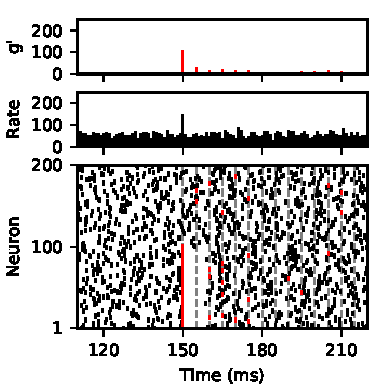
\includegraphics[width=\textwidth]{Figs/spikes_l_dt_100us.pdf}
\end{subfigure}%
\begin{subfigure}[t]{0.5\textwidth}
\caption{}\vspace{-1ex}
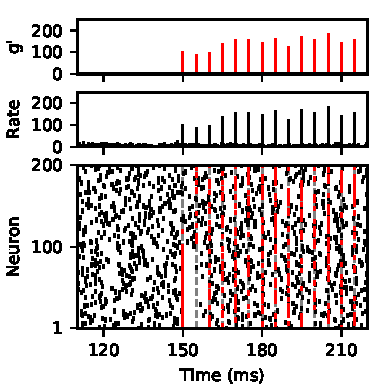
\includegraphics[width=\textwidth]{Figs/spikes_nl_dt_100us.pdf}
\end{subfigure}
\caption{\label{fig:raster}
\textbf{Propagation of synchronous spiking in linearly (A) and non-linearly (B) coupled networks.} We initiate a chain of synchronous pulses by applying external supra-threshold inputs to the first 100 neurons at time $t=\SI{150}{\milli\second}$ (red coloured spikes, grey vertical dotted lines indicate times where spikes occur as part of the chain). Top row: total size $g'$ of synchronized groups within the chain. Middle row: network rate over all neurons (rate in \si{\kilo\hertz}, bin size \SI{1}{\milli\second}). Bottom row: spiking activity of the first 200 neurons in a network of a 1000 neurons versus time.\\
Replication of Fig.~2 in \cite{Memmesheimer2012} (\url{https://doi.org/10.1371/journal.pcbi.1002384.g002}).}
\end{figure}

We first replicate a simulation showing the propagation of synchronous spiking activity in networks using linear (Fig.~\ref{fig:raster}A) and non-linear (Fig.~\ref{fig:raster}B) coupling. This figure corresponds to Fig.~2 of the original article. Given that the simulations are based on random synaptic connections and random initial conditions, we do not expect exact replication of spike times, but the qualitative features of the simulation are faithfully replicated: synchronous activity quickly dies out and disappears in the background activity for linearly coupled networks (Fig.~\ref{fig:raster}A) but is persistently propagated in non-linearly coupled networks (Fig.~\ref{fig:raster}B).

To confirm the equivalence of our network's behaviour with the original study over a wide range of synaptic connection strength we ran a grid search exploration for linearly (Fig.~\ref{fig:grid}A) and non-linearly (Fig.~\ref{fig:grid}B) coupled networks. Network behaviour is colour-coded as being part of one out of four classes: stable activity, but no persistent propagation (green); stable activity with persistent propagation (blue); unstable activity after synchronous stimulation (yellow); unstable activity before synchronous stimulation (red). For quantitative definitions, see Table~\ref{tab:color}. We run each combination of connection strengths 10 times, and combine the results to yield a color in RGB notation (values between 0 and 1 for the red, green, and blue component), according to:
\begin{equation}
R = U_1 + U_2;\quad G = E + U_2;\quad B = S,
\end{equation}
where $U_1$, and $U_2$ stand for the fraction of trials displaying unstable network activity before respectively after onset of propagation, and $S$ and $E$ for the fraction of trials displaying stable background activity with respectively without persistent propagation. We obtained this scheme directly from the authors of the original study, it was only coarsely described in the original publication. Combining individual results in this way does not necessarily lead to easily interpretable colours, but using a different scheme, e.g. colouring according to the class that occurred the most often, leads to visually similar results (not shown).

Our replication does not reproduce all details of the original plots (in particular at the top of the plots), but looks very similar on a coarse scale. Importantly, it strongly supports the original paper's main conclusion that non-linearly coupled networks have a large parameter range of stable propagation (i.e., blue-coloured points), while linearly coupled networks do not. The minor differences in our replication could be due to either our use of a clock-based simulation method, or to the slightly different initial conditions (no spikes ``in transit'').
\begin{table}
\begin{tabular}{ c  l  p{0.32\textwidth}}
  \toprule
   & Class & Definition \\
  \midrule
  $U_1$ (red) & Unstable before stimulation & $\exists t<t_\text{stim}: a_b(t) \geq 100$ \\
  $U_2$ (yellow) & Unstable after stimulation & $\exists t>t_\text{stim}: a_b(t) \geq 100$ \\
  $E$ (green) &  Stable activity, no propagation & $\forall t: a_b(t) < 100\, \wedge\, g_\text{p} < 10$\\
  $S$ (blue) & Stable activity, persistent propagation & $\forall t: a_b(t) < 100\, \wedge\, g_\text{p} \geq 10$\\
  \bottomrule
\end{tabular}
\caption{Classification of network behaviour for Fig.~\ref{fig:grid}. Here, $a_b$ refers to the background activity, the number of neurons active during a \SI{1}{\milli\second} time bin, ignoring the time steps at $t_\text{p}^k = t_\text{stim} + k\cdot\tau$, i.e. time steps that follow the synchronous stimulation by multiples of the synaptic delay. The variable $g_\text{p}$ refers to the number of successful propagations of the synchronous activity, i.e. the number of time steps $t_\text{p}^k$ where the number of active neurons exceeds the maximal background activity $a_b$.}\label{tab:color}
\end{table}

\begin{figure}
\centering
\begin{subfigure}[t]{0.5\textwidth}
\caption{}\vspace{-1ex}
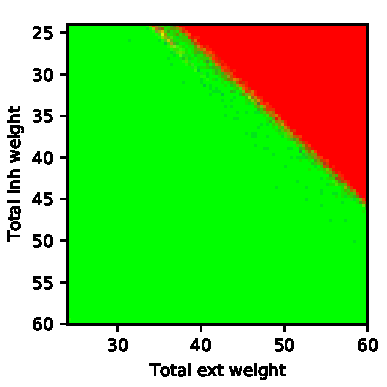
\includegraphics[width=\textwidth]{Figs/grid_l_dt_100us_mean.pdf}
\end{subfigure}%
\begin{subfigure}[t]{0.5\textwidth}
\caption{}\vspace{-1ex}
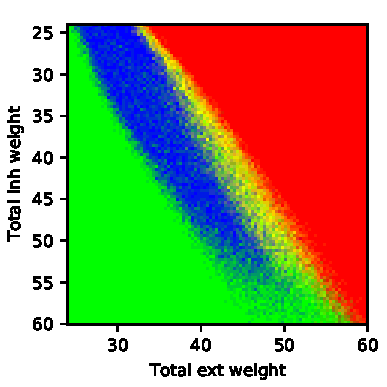
\includegraphics[width=\textwidth]{Figs/grid_nl_dt_100us_mean.pdf}
\end{subfigure}
\caption{\label{fig:grid}
\textbf{Qualitative network behaviour as a function of excitatory and inhibitory connection strength for linearly (A) and non-linearly (B) coupled networks.} For each combination, we initiated synchronous activity with 100 neurons and assessed the stability of the temporal evolution. Blue colouring indicates stable propagation of synchrony, red indicates unstable background activity before onset of propagation, yellow indicates unstable background activity after onset of propagation, and green colouring indicates the absence of propagation (see Methods for details).\\
Replication of Fig.~3a and b in \cite{Memmesheimer2012} (\url{https://doi.org/10.1371/journal.pcbi.1002384.g003})}
\end{figure}

\begin{figure}
\centering
\begin{subfigure}[t]{0.5\textwidth}
\caption{}\vspace{-1ex}
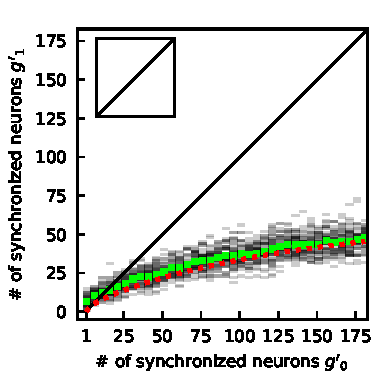
\includegraphics[width=\textwidth]{Figs/markov_l_dt_100us.pdf}
\end{subfigure}%
\begin{subfigure}[t]{0.5\textwidth}
\caption{}\vspace{-1ex}
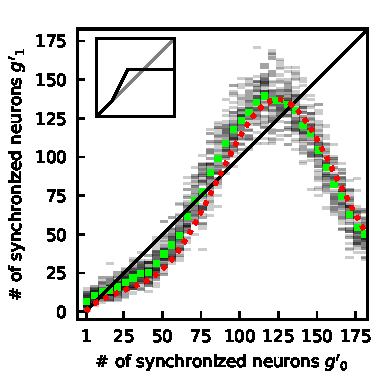
\includegraphics[width=\textwidth]{Figs/markov_nl_dt_100us.pdf}
\end{subfigure}
\caption{\label{fig:markov}
\textbf{Evolution of synchronous pulses in linearly (A) and non-linearly (B) coupled networks.} To numerically estimate the probability distribution, we show occurrences of pulse-sizes $g'_1$ in response to a pulse of size $g'_0$ by grey lines; green squares represent the corresponding mean response group sizes.\\
Replication of Fig.~4 in \cite{Memmesheimer2012} (\url{https://doi.org/10.1371/journal.pcbi.1002384.g004})}
\end{figure}

Finally, we looked at the evolution of synchronous group sizes for one combination of synaptic weights ($w_\text{ex}=w_\text{in}=\SI{0.2}{\milli\volt}$) in detail (Fig.~\ref{fig:markov}). The results confirms our previous conclusion that we can faithfully replicate the network behaviour. They match both qualitatively and quantitatively, the group size consistently declines with each iteration in linearly coupled networks (Fig.~\ref{fig:markov}A), whereas it increases for intermediate group sizes and declines otherwise in non-linearly coupled networks (Fig.~\ref{fig:markov}B). While the semi-analytic solution (red dotted line) shows a good match to the numerical results (grey lines, means as green dots), it shows some quantitative differences to the semi-analytic solution presented in Fig.~4 of the original article. In particular, our semi-analytical solution seems to mostly slightly underestimate the size of the group in the next iteration while the semi-analytical solution presented in the original article seems to slightly overestimate it.

\section*{Discussion}

We managed to qualitatively reproduce the main results of Raoul-Martin Memmes\-heimer and Marc Timme \cite{Memmesheimer2012} despite some slight quantitative differences. These difference could be due to our use of clock-based instead of event-driven simulations, as it forces all activity to a temporal grid of finite precision. We tried finer (\SI{0.05}{\milli\second}) and coarser (\SI{0.2}{\milli\second}, \SI{0.5}{\milli\second}) temporal resolutions and obtained qualitatively the same results (not shown). Another potential source for the differences is that our initial conditions do not include spikes ``in transit'' at the start of the simulation, which might further contribute to the quantitative differences we see.

The reusable code we provide with this work paves the way to future studies of networks of non-linearly coupled integrate-and-fire neurons. It gives researchers the means to verify that the original study's conclusion hold under variations of its model assumptions, such as the details of the connectivity scheme or the synaptic model. This article has already provided a first such verification, demonstrating that the original studies main findings do not critically depend on the event-based method and the entailing ``perfect time resolution''. Finally, we hope that the provided code can also serve as a basis for future studies of functional paradigms going beyond the mere propagation of synchronous activity.

\section*{Acknowledgements}
We would like to thank Raoul Martin Memmesheimer for providing implementation details about the original study. This work has received funding from the European Union’s Horizon 2020 research and innovation programme under grant agreement No 640891 (DREAM Project).

{\sffamily \small
   \printbibliography[title=References]
%}

\end{document}
